\documentclass{cumcm}


% \title{text}这里是显示在第三页的文章标题
\title{锂电池SOH预测模型设计}
% \displaytitle{text} 这里是显示在承诺书上的文章标题,注意,不能换行,如果题目特别长,要进行适当的缩写
\displaytitle{锂电池SOH预测模型设计}
% \school{text}命令用于在承诺书上显示学校名称。按要求,此处应填写全称
\school{上海交通大学}
% 以下命令分别显示队员、指导教师姓名以及队伍编号
\authorone{程云龙}
\authortwo{李羚子}
\authorthree{李汉威}
\advisor{高晓沨}
\teamnumber{130}

\begin{document}

% 这里用于打印承诺书以及编号页
 
%\newpage
\thispagestyle{empty} %取消当前页码
{\Large \heiti \begin{center}\the\year~高教社杯全国大学生数学建模竞赛\par\vspace{0.5\ccwd}\par
{\ziju{1}承诺书}\end{center}\par\vspace{1\ccwd}\par}
\renewcommand{\baselinestretch}{1.5}\normalsize
{\zihao{-4}%
我们仔细阅读了中国大学生数学建模竞赛的竞赛规则。\par
我们完全明白,在竞赛开始后参赛队员不能以任何方式(包括电话、电子邮件、网上咨询等)
与队外的任何人(包括指导教师)研究、讨论与赛题有关的问题。\par
我们知道,抄袭别人的成果是违反竞赛规则的, 如果引用别人的成果或其他公开的资料
(包括网上查到的资料),必须按照规定的参考文献的表述方式在正文引用处和参考文献中明确列出。\par
我们郑重承诺,严格遵守竞赛规则,以保证竞赛的公正、公平性。如有违反竞赛规则的行为,我们将受到严肃处理。\par
\par\vspace{2\ccwd}\par
\raisebox{1ex}[0pt]{我们参赛的题目是:}\vbox{\hbox to11.4cm{\hfil \the\displaytitle \hfil}
        \protect\vspace{0.6truemm}\relax
        \hrule depth0pt height0.15truemm width11.4cm}\par
\vspace{1mm}
\raisebox{1ex}[0pt]{我们的参赛报名号为(如果赛区设置报名号的话):}\vbox{\hbox to5.75cm{\hfil \the \teamnumber  \hfil}
        \protect\vspace{0.6truemm}\relax
        \hrule depth0pt height0.15truemm width5.75cm}\par
\vspace{1mm}
\raisebox{1ex}[0pt]{所属学校(请填写完整的全名):}\vbox{\hbox to9.12cm{\hfill \the\school \hfill}
        \protect\vspace{0.6truemm}\relax
        \hrule depth0pt height0.15truemm width9.12cm}\par
\begin{tabular}{lcp{8.82cm}c}
\hspace{-2.1mm}\raisebox{-1mm}[0pt]{参赛队员(打印并签名): }&\raisebox{-1mm}[0pt]{1、}& \raisebox{-1mm}[0pt]{\the\authorone\hfill{}}& \\ \cline{3-3}
   &\raisebox{-1mm}[0pt]{2、}& \raisebox{-1mm}[0pt]{\the\authortwo\hfill{}}& \\ \cline{3-3}
   &\raisebox{-1mm}[0pt]{3、}& \raisebox{-1mm}[0pt]{\the\authorthree\hfill{}}& \\ \cline{3-3}
\end{tabular}
\par
\vspace{10mm}
\raisebox{1ex}[0pt]{指导教师或指导教师组负责人(打印并签名):}\vbox{\hbox to6.65cm{\the\advisor \hfil}
        \protect\vspace{0.6truemm}\relax
        \hrule depth0pt height0.15truemm width6.65cm}\par
\vspace{5mm}
{}\hspace{10cm}日期:\hrulefill\hrulefill 年\hrulefill 月 \hrulefill 日
\par
\vspace{2cm}
\hrulefill\par\vspace{2\ccwd}\par
赛区评阅编号(由赛区组委会评阅前进行编号):
}
\renewcommand{\baselinestretch}{1.3}\normalsize
\newpage
\thispagestyle{empty} %取消当前页码
{\Large \heiti \begin{center}\the\year~高教社杯全国大学生数学建模竞赛\par\vspace{0.5\ccwd}\par
{\ziju{1}编号专用页}\end{center}\par\vspace{1\ccwd}\par}
{\zihao{-4}%
\par\vfill
赛区评阅编号(由赛区组委会评阅前进行编号):\par\vfill\vfill

赛区评阅记录(可供赛区评阅时使用):\vspace{1\ccwd}

\begin{center}
\resizebox{.9\textwidth}{!}{
\begin{tabular}{|c|*{10}{p{.09\textwidth}|}}
\hline
\makecell{评\\阅\\人}&&&&&&&&&&\\
\hline
\makecell{评\\分}&&&&&&&&&&\\
\hline
\makecell{备\\注}&&&&&&&&&&\\
\hline
\end{tabular}
}
\end{center}\vspace{1\ccwd}

全国统一编号(由赛区组委会送交全国前编号):\par\vfill\vfill

全国评阅编号(由全国组委会评阅前进行编号):\par\vfill\vfill\vfill
}
\renewcommand{\baselinestretch}{1.3}\normalsize

\newpage

\begin{minipage}{0.9\textwidth}
\centering\LARGE\textbf{锂电池SOH预测模型设计}
\end{minipage}
\begin{abstract}
本题题意在于通过对测试数据充足的锂电池建立SOH模型,找出可测数据与电池SOH之间的关系,并使模型适用于不同的锂电池,进而完成测试数据较少的锂电池SOH预测。\par
\textbf{针对问题一}\quad 我们通过采用电化学阻抗谱法和电压曲线拟合法,分别找出电池电阻、恒流充电电压与电池SOH之间的关系,从而建立预测模型。然后利用层次分析法,找出内阻与电压两个因素对电池SOH影响所占权重,加权计算出


\textbf{关键词} \quad MATLAB \quad 电化学阻抗谱法  \quad 电压曲线拟合法
\end{abstract}

\newpage
\section{问题重述}
\subsection{问题背景}
电池是一种能量转化与储存的装置,它通过反应可将化学能或物理能转化为电能,从而得到具有稳定电压、长时间稳定供电的电流。作为众多移动终端的动力单元及绿色环保电池的首选,锂离子电池在电池界具有举足轻重的地位,并在各种电子设备中得到了越来越广泛的应用。其在便携式设备、储备电源、卫星、电动汽车等领域,更是具有广阔的前景。
\subsection{问题的提出(题目重述)}
随着使用情况的增多,锂离子电池会逐渐老化,我们通常采用SOH(锂电池放电容量与锂电池额定容量的比值)表示锂离子电池的老化程度。为了保证设备的稳定,预测锂电池的SOH便具有了重要的意义。然而不同类型的锂电池,其测试数据的多少会有不同。要求利用一个测试数据充足的锂电池SOH预测模型,通过数学建模方法转化,完成测试数据较少的锂电池SOH预测。

\begin{itemize}
\item \textbf{任务一} \quad 利用源数据中B0007号锂电池全部循环测试的充放电参数(电压、电流等)建模预测源数据中B0005号锂电池SOH,计算真实SOH值与预测值的均方根误差。
\item \textbf{任务二} \quad 取cell1、cell3、cell7、cell8中前一半数据,结合任务一B0007号锂电池的模型再次建模,对这四种电池中另一半缺失数据的锂电池SOH进行预测,计算真实SOH值与预测值的均方根误差。
\end{itemize}

\section{模型假设}
\begin{enumerate}
\item 在本题所给数据中,环境温度恒为$24^\circ$C,所以外界环境温度对电池SOH的影响不予考虑。
\item 不考虑恒压充电情况。
\item 不考虑充放电电流对电池SOH值影响。
\item 将电池EIS、恒流充电电压作为电池SOH的两大影响因素。
\end{enumerate}
\section{假设说明}
\begin{enumerate}
\item EIS为电池老化过程中阻抗谱变化。
%\item 由参考文献\cite{}可知,在恒压充电情况下,电池SOH值改变较小,可忽略,仅考虑恒流充电情况。
\item 考虑电池在放电过程中,放电电流、温度等因素较为复杂,而充电过程情况较为稳定,因此选用电池充电电压曲线拟合估算。
%\item 由论文\cite{}可知,电池EIS会随着电池老化而发生相应改变,说明EIS变化与电池SOH衰减具有相关性。
\end{enumerate}


\section{问题分析}
对于问题一和问题二,可采用同样的方法进行建模。\par
由题目所给测试数据及所查参考文献,对于锂电池老化机理分析,我们仅考虑电池EIS及恒压充电电压两个因素的改变对电池SOH值的影响。%论文\cite{}
对阻抗参数与电池老化规律进行了分析,并验证了基于阻抗法估算电池SOH的可行性。通过电化学阻抗谱模型可以建立电池EIS与电池老化过程中相应内部参数之间的联系;通过电压曲线拟合法得出充电电压与电池SOH的关系。然后利用层次分析法,找出两因素的影响权重,加权计算得到最终的SOH预测结果,算出其与真实SOH的均方根误差,进行比较。
\subsection{问题一分析}
\begin{enumerate}[(1)]
\item \textbf{电化学阻抗谱法}\par
本题所给测试数据中,采用循环充放电方式对BOOO7号样本电池老化试验,我们可得出随着循环次数的增加,电池SOH衰减曲线,如图所示:
\begin{figure}[H]
\centering
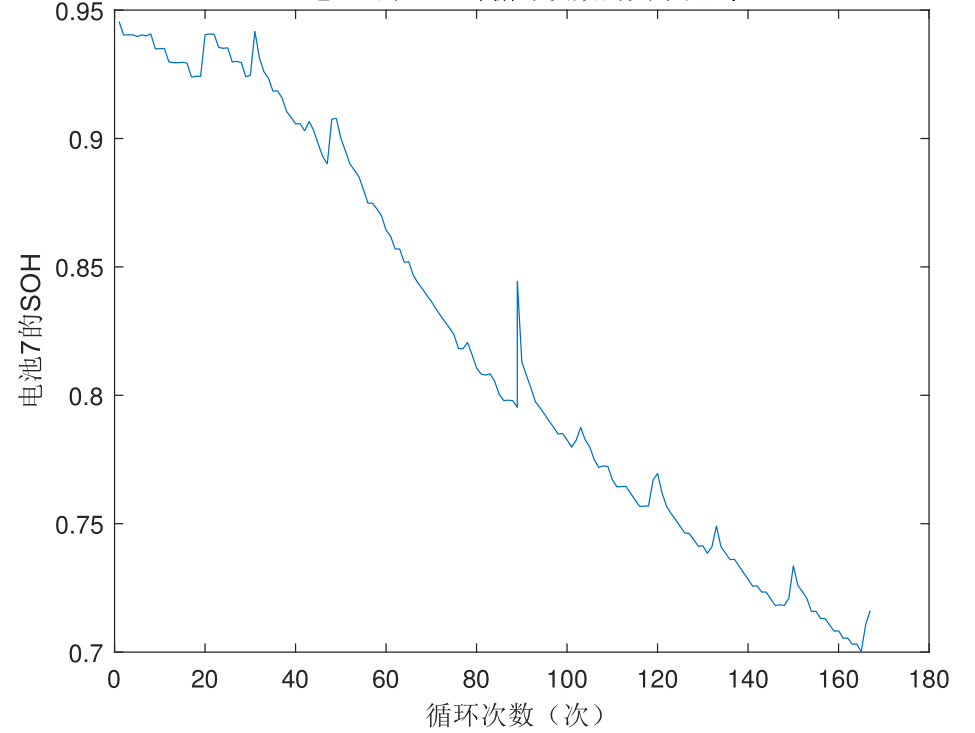
\includegraphics[width=0.8\textwidth]{img/7-SOH-cycle.png}
\caption{电池B0007的SOH与循环次数关系曲线}\label{figure-a}
\end{figure}
在循环次数内,SOH值基本呈线性下降,属正常老化。同时,电池内阻随着循环次数增加而逐步增加,可得到如图所示结果。
\begin{figure}[H]
\centering
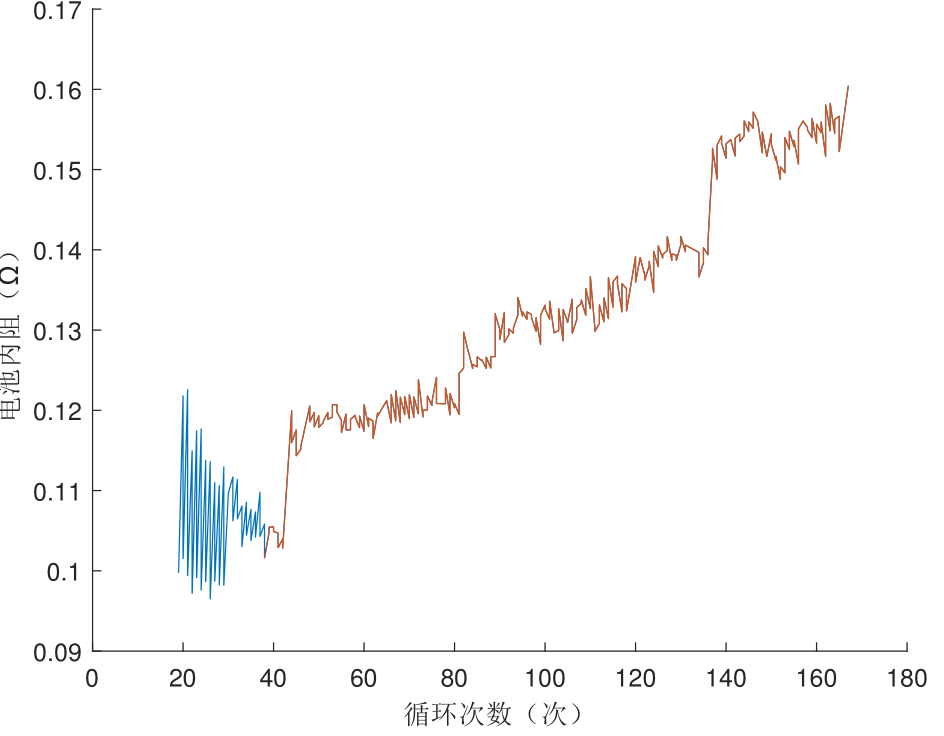
\includegraphics[width=0.8\textwidth]{img/R-cycle.png}
\caption{电池B0007的内阻与循环次数关系曲线}\label{figure-b}
\end{figure}

我们发现在电池循环前期,随着循环次数的增加,电池电阻缓慢下降,当循环试验进行到后期。随着循环次数的增加,电池内阻会有很大程度的下降。其中,前面波动较大是由于新电池刚开始充电时性能不稳定造成的,所以可把这一部分不考虑在内,只考虑循环后期电池状况稳定的情况。对余下曲线进行拟合,如图所示:\par
\begin{figure}[H]
\centering
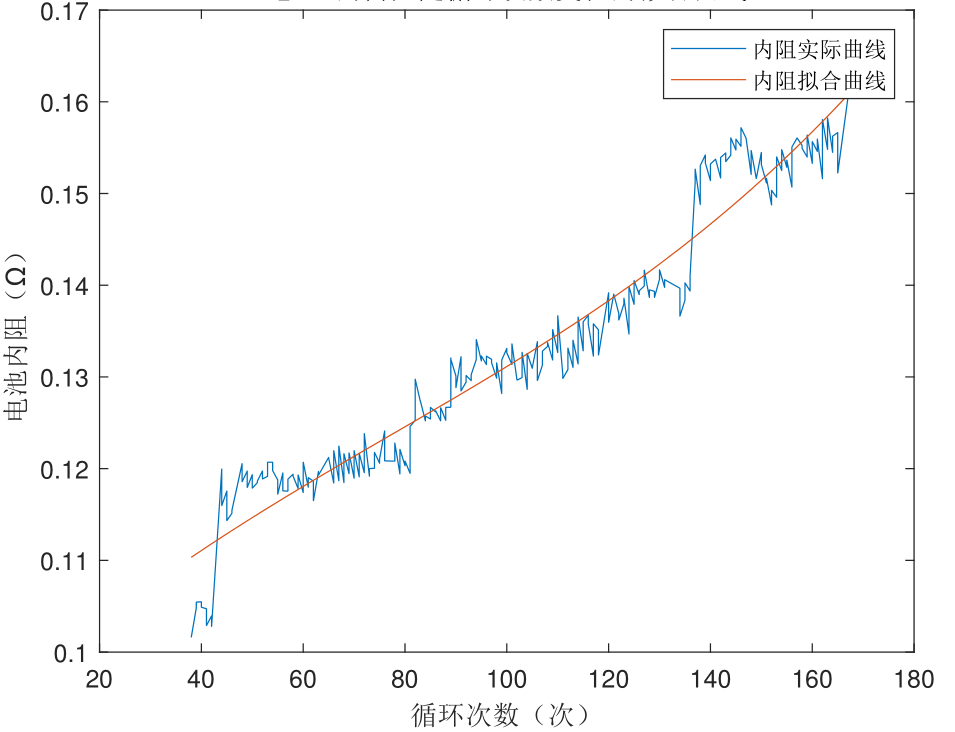
\includegraphics[width=0.8\textwidth]{img/R-cycle-fit.png}
\caption{电池B0007的内阻与循环次数的拟合曲线}
\end{figure}
所以,所给数据符合电化学阻抗谱法适用条件。

\item \textbf{电压曲线拟合法}
\end{enumerate}
\subsection{问题二分析}



\section{问题的解答}
\subsection{问题1的解答}
\begin{enumerate}[(1)]
\item \textbf{电化学阻抗谱法}
我们用电阻测试结果表示SOH,可获得如图的SOH和电池电阻关系图,分析数据可知,电池SOH随着电阻老化呈单调下降,采用四次拟合的方法,我们可近似计算电池SOH老化规律曲线
\begin{figure}[H]
\centering
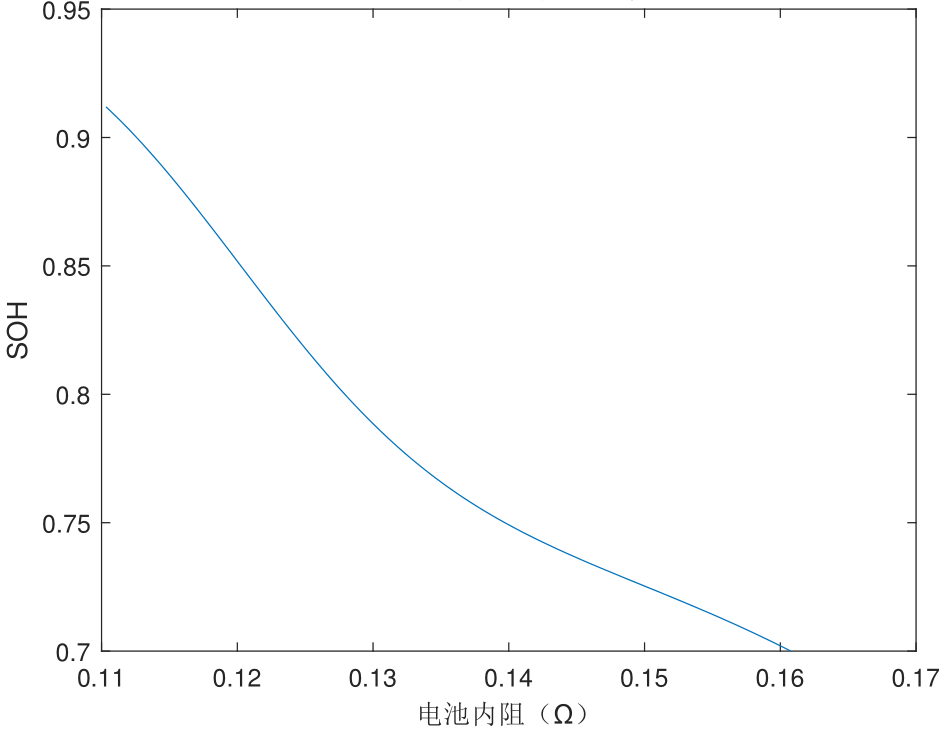
\includegraphics[width=0.8\textwidth]{img/SOH-R-fit.png}
\caption{电池B0007的SOH与其内阻变化曲线}
\end{figure}
通过MATLAB拟合求解,可得到相关系数为$0.9483$,表明两者相关性较强,可用该模型来预测B0005电池SOH。代入目标数据求得B0005预测SOH与真实值之间的均方根误差为$0.0296j$。
\item \textbf{电压曲线拟合法}

\end{enumerate}
\subsection{问题2的解答}


\section{模型总结}

\subsection{模型优点}

\subsection{模型缺点}


\bibliographystyle{plain}
\bibliography{ref}

\newpage
\appendix
\textbf{附录}
\section{模型求解代码}

\end{document}

